\section{System Design and Architecture}
\label{sec:architecture}

\subsection{Component Responsibilities}

The extension preserves the principal DecMed components and changes their authorization responsibilities. The Patient Client creates the initial consent request, signs the patient's nonce, reviews delegation history, and initiates revocation. The Hospital Client is used by records personnel and medical actors to retrieve encrypted access metadata, access permitted record segments, and request delegation. The PRE Server issues root Macaroons, validates attenuation and data requests, enforces category and institutional constraints, and performs re-encryption; in the PAP/PIP/PDP/PEP mapping of Section~\ref{sec:approach}, it colocates PDP and PEP. Redis stores ephemeral PRE material and revocation keys. IOTA stores personnel state, segment metadata, encrypted access metadata, and delegation audit records, while IPFS stores encrypted segment objects.

Fig.~\ref{fig:decmed-data-flow} shows the DecMed system context retained by the extension. Patient, hospital, and ministry actors remain outside the DecMed boundary, while encrypted record objects and on-chain transactions flow to IPFS and IOTA, respectively. Within the boundary, hospital requests pass through the proxy API and authentication/access-control path before medical-record management can invoke PRE or interact with the stores. The extension therefore does not replace DecMed's storage or PRE architecture; it narrows the conditions under which those paths execute.

\begin{figure*}[t]
	\centering
	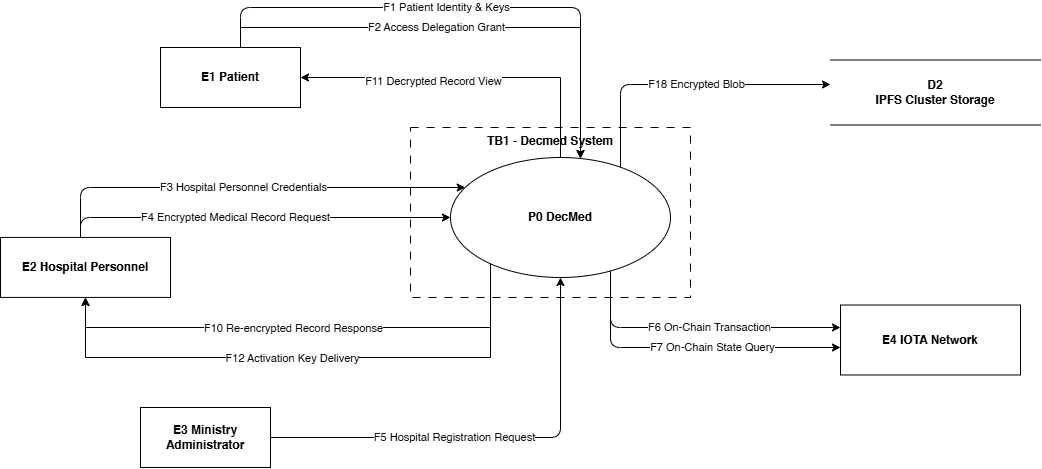
\includegraphics[width=0.9\textwidth]{resources/paper/decmed-data-flow.png}
	\caption{DecMed system context retained by the access-control extension, with patient and institutional actors, encrypted IPFS storage, and IOTA transactions (thesis artifact).}
	\label{fig:decmed-data-flow}
\end{figure*}

\subsection{Initial Grant}

The patient remains the authority for the first grant. Records personnel display a QR value containing the hospital identifier, IOTA wallet address, and PRE public key. After scanning it, the Patient Client checks the personnel record on IOTA and lets the patient choose outpatient or inpatient service, read/update mode, and expiry. The client obtains a nonce from PRE and signs it with the patient's IOTA key. PRE verifies the patient and confirms that the recipient is active administrative personnel at the selected hospital.

PRE then issues separate read and update Macaroons. A read token initially covers the implemented datasets and functions; an update token is limited to the selected encounter dataset plus laboratory and pharmacy and is bound to a newly generated \texttt{related\_rme\_id}. Both carry the hospital, recipient root subject, expiration, and maximum delegation depth. Broad root scope does not itself authorize records personnel to write clinical data because every request is also checked against their on-chain role.

The Patient Client generates the PRE data seed and encrypts it for the initial recipient. The token, token hash, encrypted seed, and access metadata are encrypted with the recipient's PRE public key and recorded through the IOTA \texttt{create\_access} function. PRE stores the associated re-encryption material in Redis with a lifetime derived from the access expiry. Thus, the ledger distributes encrypted access metadata rather than a plaintext bearer token.

\subsection{Delegation and Request Verification}

After the initial grant, records personnel may delegate to a nurse or physician. A physician may further delegate a restricted capability to laboratory personnel or a pharmacist. The root token has depth two; the first child has one remaining level, and the second-level child has zero. Presets implement task-specific scopes: a nurse receives initial-examination functions, laboratory personnel receive supporting-examination read scope and laboratory write scope, and a pharmacist receives therapy/prescription read scope and pharmacy write scope.

The delegator's Hospital Client obtains the candidate's public information from IOTA, decrypts the existing data seed, and re-encrypts it for the delegatee. It sends the parent token, requested scope and expiry, actor addresses, and a wallet-signed \texttt{DelegationRequestProofContext} to PRE. PRE authenticates the parent, checks all parent and ancestor revocation keys, verifies the delegator signature, computes the effective capability, and obtains an IOTA access snapshot. The snapshot confirms active accounts, a common hospital, parent validity, current depth, and the absence of a conflicting active delegation for the same recipient subrole. If the request is monotonic, PRE appends the child caveats and returns the child token and hash.

The client signs a \texttt{DelegationProofContext}, packages the child token, proof, re-encrypted seed, and metadata, and encrypts the package for the delegatee. The IOTA \texttt{create\_delegated\_access} function records the encrypted package and an audit entry containing delegator, root subject, delegatee, mode, episode, depth, parent and child token hashes, and expiry. The patient is not part of these steps, but the client, PRE Server, IOTA, Redis, and network are still required.

To use the grant, the delegatee decrypts its access package locally and sends the Macaroon with a request. PRE reconstructs the ordered delegation chain; the last \texttt{delegated\_to} value is the active subject. It then checks chained-HMAC authenticity, expiration, depth, revocation, actor role/subrole on IOTA, and segment context. A wallet proof signs the token identifier, patient, episode, operation, segment, dataset, function, and timestamp. Only after the proof matches the active subject does a read trigger IPFS retrieval and Umbral re-encryption, or a write store ciphertext in IPFS and metadata in IOTA.

\section{Implementation}
\label{sec:implementation}

The prototype was implemented mainly in Rust and retained the existing Tauri clients and IOTA Move contracts. Fig.~\ref{fig:package-diagram} summarizes the shared packages introduced for the extension. \texttt{decmed-rme-segment} defines category enums, segment data and metadata, validation, and integrity-hash utilities. \texttt{decmed-macaroon-auth} wraps the adapted open-source \texttt{macaroon} crate with DecMed issuance, caveat parsing, effective-capability calculation, attenuation, chain construction, wallet-proof context, and revocation-key functions. The Patient Client, Hospital Client, and PRE Server consequently share the same segment schema; the Hospital Client and PRE Server also share authorization types.

\begin{figure*}[t]
	\centering
	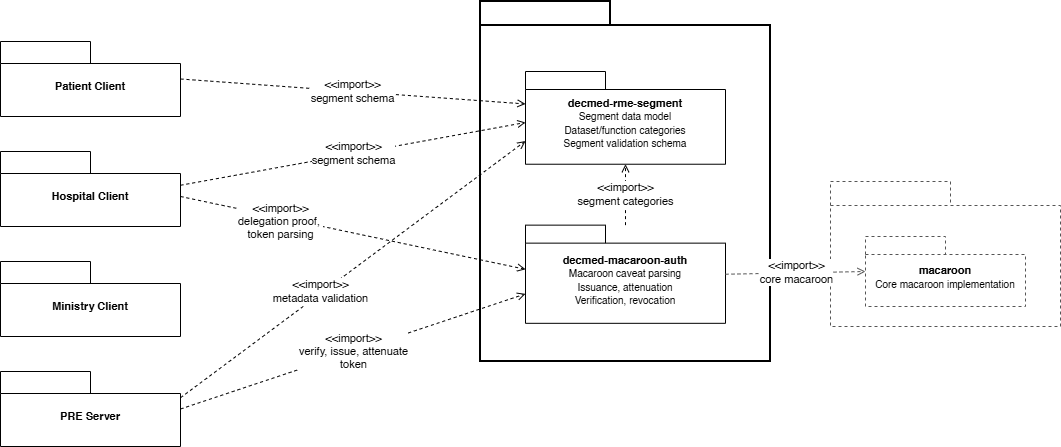
\includegraphics[width=0.9\textwidth]{resources/paper/implementation-package-diagram.png}
	\caption{Shared implementation packages for segmentation and Macaroon authorization (thesis artifact).}
	\label{fig:package-diagram}
\end{figure*}

Each \texttt{RmeSegmentData} object contains segment and episode identifiers, categories, patient and author addresses, service date, payload, and payload hash. After client-side encryption and IPFS upload, \texttt{RmeSegmentMetadata} retains the contextual fields together with the IPFS CID, ciphertext integrity hash, PRE capsule, encrypted key/nonce, hospital identifier, and creation time. The metadata is serialized as base64-encoded JSON inside the existing flat IOTA metadata list, maintaining compatibility while making categories available to PRE.

Authorization is implemented as PRE middleware plus operation-specific handlers. The middleware deserializes the bearer Macaroon, validates its chained HMAC, rejects unknown caveats, builds \texttt{EffectiveCapability} and \texttt{DelegationChain}, checks expiry and depth, and queries Redis using keys of the form \texttt{revoked:token:<hash>}. Read and write handlers then validate the metadata or payload preview against patient, episode, hospital, dataset, function, and operation constraints. They obtain the active actor's institutional role from the Move contract and verify the wallet signature. The accepted proof window is five minutes. On a read without a proof, PRE returns an authorization response containing the canonical context so the client can sign and retry.

Revocation combines immediate enforcement and durable state. The Patient Client first invokes the Move revocation path, which marks access and downstream delegations as revoked and records an audit event. It then asks PRE to store token hashes in Redis until token expiry and delete associated re-encryption material. When a descendant is presented, PRE checks its own hash and every \texttt{parent\_token\_hash}; a revoked ancestor therefore invalidates the derived request.

\section{Evaluation}
\label{sec:evaluation}

\subsection{Environment and Method}

The evaluation used a proof-of-concept deployment rather than an operational hospital system. Patient, hospital, and ministry clients and the PRE Server ran on Ubuntu 24.04.4 under WSL2 on an Intel Core i5-11400H host; WSL2 was allocated three physical cores, six logical threads, and 8~GB of the host's 16~GB RAM. Two Ubuntu 24.04.4 VPS instances, each with eight vCPUs and 8~GB RAM, hosted supporting services. The three-peer IPFS cluster, IOTA Gas Station, and IOTA Localnet deployment were placed on the VPS infrastructure.

Evaluation traced each stated requirement to implementation evidence and a test scenario. Twelve functional tests (\texttt{P-KF-01}--\texttt{P-KF-12}) were executed manually over outpatient and inpatient workflows. The inpatient path additionally exercised the discharge-planning segment. Sixteen nonfunctional tests (\texttt{P-KNF-01}--\texttt{P-KNF-16}) combined Rust unit/integration tests run with \texttt{cargo test} and client-level scenarios. These tests concern authorization correctness, traceability, and selected negative cases; they are not penetration tests or performance benchmarks.

Table~\ref{tab:evaluation-summary} groups the documented scenarios without treating each user-interface step as a separate scientific result. Within the evaluated test scenarios and prototype boundaries, the tested functional and nonfunctional requirements are considered fulfilled.

\begin{table*}[t]
	\caption{Grouped Evaluation Evidence}
	\label{tab:evaluation-summary}
	\centering
	\small
	\setlength{\tabcolsep}{4pt}
	\begin{tabular}{@{}p{0.18\textwidth}p{0.18\textwidth}p{0.48\textwidth}p{0.10\textwidth}@{}}
		\toprule
		\textbf{Category}                                                                                                                              & \textbf{Test IDs} & \textbf{Tested behavior and documented outcome} & \textbf{Status} \\
		\midrule
		Initial access and delegation                                                                                                                  &
		\texttt{P-KF-01}--\texttt{03}, \texttt{06}, \texttt{09}                                                                                        &
		Patient-to-records-personnel tokens and narrower nurse, physician, laboratory, and pharmacy child tokens were created for the clinical flow.   &
		Fulfilled                                                                                                                                                                                                                              \\
		Role-scoped clinical operations                                                                                                                &
		\texttt{P-KF-04}, \texttt{05}, \texttt{07}, \texttt{08}, \texttt{10}                                                                           &
		Nurse initial-examination, physician clinical, laboratory, and pharmacy read/write operations processed their corresponding segments.          &
		Fulfilled                                                                                                                                                                                                                              \\
		Patient control and traceability                                                                                                               &
		\texttt{P-KF-11}, \texttt{12}                                                                                                                  &
		The patient viewed the delegation history and revoked access; the delegatee could no longer access the record.                                 &
		Fulfilled                                                                                                                                                                                                                              \\
		Out-of-scope data                                                                                                                              &
		\texttt{P-KNF-01}, \texttt{02}                                                                                                                 &
		PRE rejected a laboratory segment outside token caveats, and a pharmacist client did not expose laboratory data.                               &
		Fulfilled                                                                                                                                                                                                                              \\
		Monotonic attenuation                                                                                                                          &
		\texttt{P-KNF-03}--\texttt{06}                                                                                                                 &
		Requests that added a write function/dataset, increased depth, or extended expiry beyond the parent were rejected.                             &
		Fulfilled                                                                                                                                                                                                                              \\
		Token, chain, and wallet validity                                                                                                              &
		\texttt{P-KNF-07}--\texttt{09}, \texttt{13}                                                                                                    &
		Expired tokens, broken delegation chains, missing wallet proofs, and proofs from a non-active actor were rejected.                             &
		Fulfilled                                                                                                                                                                                                                              \\
		Audit and revocation enforcement                                                                                                               &
		\texttt{P-KNF-10}--\texttt{12}                                                                                                                 &
		Delegation details were displayed; a matching revocation key rejected the token, and root revocation removed active root and delegated access. &
		Fulfilled                                                                                                                                                                                                                              \\
		Integrity and on-chain confidentiality constraints                                                                                             &
		\texttt{P-KNF-14}--\texttt{16}                                                                                                                 &
		Mismatched ciphertext integrity hashes were rejected, and clinical plaintext was not stored in on-chain metadata under the tested conditions.  &
		Fulfilled                                                                                                                                                                                                                              \\
		\bottomrule
	\end{tabular}
\end{table*}

\subsection{Interpretation of Results}

The positive scenarios establish an end-to-end path from an initial patient grant to task-specific access by four clinical actor types. They also connect segmentation to observable operations: the nurse writes initial examination data, the laboratory actor reads a supporting request and writes laboratory results, and the pharmacist reads prescription-related data and writes pharmacy service data. This evidence supports functional integration of category-aware authorization; it does not quantify usability or clinical effectiveness.

The negative scenarios directly exercise the main attenuation and requester-binding invariants. Dataset/function expansion, increased depth, and later child expiry were rejected. Separate cases rejected an expired token, a discontinuous delegation chain, a missing wallet signature, and a physician signature presented for a laboratory-active token. Revocation tests covered both direct token-hash lookup and use after patient-initiated chain revocation. Together, these results support correctness of the implemented authorization rules within the tested cases. They do not demonstrate resistance to all attacks, formal cryptographic correctness, or behavior under high concurrency.

\section{Discussion}
\label{sec:discussion}

The results address the central mismatch in the earlier design: a PBAC-derived granular token now has a granular storage object against which it can be enforced. PRE compares caveat intersections with on-chain segment metadata before returning re-encryption output, so an unauthorized category is rejected before the client obtains decryptable material. Institutional subrole checks further prevent a syntactically broad update token from authorizing a professional operation outside the actor's implemented responsibility. The existing DecMed role identifier \texttt{MedicalPersonnel} continues to represent several healthcare actors; subroles distinguish nurses, physicians, laboratory personnel, and pharmacists.

PRE-mediated attenuation reduces repeated patient interaction while preserving patient control at two points: the patient authorizes the root grant and can revoke its chain. Macaroons conceptually support attenuation without the original issuer; in this system, child tokens are still formed online by the PRE Server. Delegation is therefore free of further patient involvement, but it remains a distributed transaction involving PRE validation, encrypted metadata delivery through IOTA, Redis state, and client cryptography. This improves workflow continuity only when those components are available.

PRE is a material trust and availability boundary, not the policy author. It holds the Macaroon root key, computes effective capability from PBAC-mapped caveats, validates wallets and on-chain roles, and gates re-encryption. Redis availability affects revocation and PRE material; IOTA availability affects identity, access, and audit state; IPFS availability affects ciphertext retrieval. The evaluation did not benchmark these dependencies or test large-scale failure behavior.

Other limitations follow the implemented scope. The prototype covers outpatient, inpatient, laboratory, and pharmacy datasets, represents segment payloads as text, and fixes delegation depth at two. It was evaluated locally and on VPS-hosted support services, not against a production hospital information system. The evaluation focuses on functional and authorization behavior rather than throughput, availability, scalability, broad adversarial testing, or a formal security proof; cryptographic properties are assumed from the selected libraries and schemes. Emergency access, the emergency-department dataset, and break-glass mechanisms are outside the study and are not contributions of this work.

\section{Conclusion}
\label{sec:conclusion}

This work extended DecMed with a PBAC authorization model, category-based EMR segmentation, and Macaroon capabilities whose caveats constrain operation, patient, episode, hospital, data scope, expiry, and delegation chain. PRE-mediated attenuation prevents a requested child from exceeding its parent and supports delegation among healthcare actors without further patient involvement, while wallet proof, role/subrole validation, Redis revocation, and IOTA audit records bind the capability to the implemented workflow. Across 12 functional tests (\texttt{P-KF-01}--\texttt{P-KF-12}) and 16 nonfunctional tests (\texttt{P-KNF-01}--\texttt{P-KNF-16}), the tested requirements are considered fulfilled within the evaluated prototype scope, and the tested out-of-scope, non-monotonic, expired, malformed-chain, wallet-invalid, and revoked cases were rejected.

The evidence supports functional correctness for the evaluated prototype, not a general claim of security or efficiency. Future work should validate the design in hospital-integrated and inter-facility workflows, add emergency/break-glass scenarios, map segments to SATUSEHAT/FHIR representations, and evaluate performance, availability, scalability, and security more extensively.
